\documentclass[a4paper,12pt]{report}
\usepackage[utf8]{inputenc}
\usepackage{enumitem} %permite el uso de letras para enumerar
\usepackage{graphicx} %para las imágenes
\usepackage{float} %para fijar las imágenes
\usepackage{booktabs} %para fijar las imágenes
\renewcommand{\arraystretch}{2} % Escala la altura de las filas

\usepackage{amsmath}%para entornos de alineación
\usepackage{amsfonts}%para las letras lindas de matemática
\usepackage{xfrac}%para fracciones chiquitas
\allowdisplaybreaks
\setlength{\jot}{8pt}%modifica el interlineado

\usepackage{tikz} %Librería para gráficos
\usetikzlibrary{calc, arrows.meta, positioning}

\usepackage[a4paper, %margenes de pagina
  left=2.5cm,
  right=2.5cm,
  top=2cm,
  bottom=2cm,
  includehead
]{geometry}

\usepackage{fancyhdr}
\pagestyle{fancy}
\lhead{UTN-FRC}
\chead{Dispisitivos Electronicos I}
\rhead{3R2}
\cfoot{\thepage}
\setlength{\headwidth}{\textwidth} % Hace que el ancho del encabezado coincida con el ancho del texto
\setlength{\headheight}{15pt}  % Ajusta la altura del encabezado
\setlength{\headsep}{20pt}     % Ajusta la separación entre el encabezado y el contenido

\usepackage{titlesec}
\titleformat{\chapter}[display]{\normalfont\Large\bfseries}{}{0pt}{}
\titlespacing*{\chapter}{10pt}{-45pt}{10pt}

\usepackage{etoolbox} 
\makeatletter
\patchcmd{\chapter}{\thispagestyle{plain}}{\thispagestyle{fancy}}{}{} %Muestra encabezado en las paginas con \chapter
\makeatother

%Comandos de fake section y fake sub section, para poder agregar secciones al indice
\newcommand{\fs}[1]{%
  \par\refstepcounter{section}% Increase section counter
  \sectionmark{#1}% Add section mark (header)
  \addcontentsline{toc}{section}{\protect\numberline{\thechapter.\alph{section}}#1}% Add section to ToC
}
\newcommand{\fss}[1]{%
  \par\refstepcounter{subsection}% Increase subsection counter
  \subsectionmark{#1}% Add subsection mark (header)
  \addcontentsline{toc}{subsection}{\protect\numberline{\alph{subsection}}#1}% Add subsection to ToC
}

\renewcommand{\contentsname}{Tabla de Contenidos}

\usepackage{afterpage}
\newcommand\myemptypage{
  \newpage
  \null
  \thispagestyle{empty}
  \addtocounter{page}{-1}
  \newpage
}

\usepackage{circuitikz}

\title{%
\setlength{\headwidth}{\textwidth} % Hace que el encabezado tenga el mismo ancho que el contenido
\setlength{\headheight}{15pt}  % Ajusta la altura del encabezado
\setlength{\headsep}{10pt}     % Ajusta la separación entre el encabezado y el contenido
  \fontsize{25}{0}\selectfont Universidad Tecnológica Nacional \\
  \fontsize{22}{30}\selectfont Dispositivos Electronicos I \\
  \fontsize{20}{25}\selectfont Trabajo Practico N° 1
}
\author{
  Santino Noccetti - 405927\\
  Franco Palombo - 401910\\
}
\date{08 / 04 / 2025}

\begin{document}

  \maketitle

  \myemptypage

  \tableofcontents
  \thispagestyle{plain}

  \myemptypage

  \chapter{Introduccion}
    Introduccion.


  \chapter{Actividad Practica}
    \section{Calculos}
    \vspace{-0.6cm}
      \begin{figure}[h]
        \centering
        \begin{minipage}{0.7\textwidth}
          \centering
          \begin{circuitikz}[american voltages]
              % nodos
              \draw
                (0, -1) to [V=$V_s$, on grid, invert]                   (0, 3)
                        to [short, -, i>^=$I_t$, on grid]               (1, 3)
                        to [R=$R_1$, v=$V_{R_1}$, on grid]              (4, 3)
                        to [short, -*, on grid]                         (5, 3)
                        to [short, -, on grid]                          (8, 3)
                        to [short, -, i>^=$I_3$, on grid]               (8, 2)
                        to [R=$R_3$, v=$V_{R_3}$, on grid]              (8, 0)
                        to [short, -, on grid]                          (8, -1)
                        to [short, -*, on grid]                         (5, -1)
                        to [short, -, on grid]                          (0, -1)
                        to [short, -, on grid]                          (0, -1)
                (5, 3)  to [short, -, i>^=$I_2$, on grid]               (5, 2)
                        to [R=$R_2$, v=$V_{R_2}$, on grid]              (5, 0)
                        to [short, -, on grid]                          (5, -1)
                ;
          \end{circuitikz}
        \end{minipage}
        \centering
        \begin{minipage}{0.2\textwidth}
          \centering
          \begin{align*}
            V_s &= 10V\\
            R_1 &= 10K\Omega\\
            R_2 &= 4K7\Omega\\
            R_3 &= 3K3\Omega
          \end{align*}
        \end{minipage}
      \end{figure}

      Ecuaciones del Circuito:
      \begin{gather*}
        \begin{cases}
          M_1: &-V_s + V_{R_1} + V_{R_2} = 0\\
          M_2: &-V_s + V_{R_1} + V_{R_3} = 0\\
          &I_2 + I_3 = I_t
        \end{cases}
      \end{gather*}

      Sabiendo que, por ley de Ohm, la caida de tension en cualquier resistor es:
      \begin{equation}
        V_R = R I
      \end{equation}
      donde $R$ es la resistencia de dicho resistor, e $I$ la intensidad de corriente que pasa por ese resistor,
      podemos entonces despejar la caida de tension en la $R_1$ reemplazando la caida de tension de la $R_2$ en la ec.
      de la malla $M_1$:
      \begin{figure}[!h]
        \centering
        \begin{minipage}{0.6\textwidth}
          \centering
          \begin{align*}
            -V_s + V_{R_1} + V_{R_2} &= 0\\
            -V_s + V_{R_1} + R_2 I_2 &= 0\\
            -V_s + V_{R_1} + R_2 (I_t - I_3) &= 0\tag*{\hfill(\ref{i2_sub})}\\
            -V_s + V_{R_1} + R_2 \left(\frac{V_{R_1}}{R_1} - \frac{V_{R_3}}{R_3}\right) &= 0\tag*{\hfill(\ref{it_sub})(\ref{i3_sub})}\\
            -V_s + V_{R_1} + V_{R_1} \frac{R_2}{R_1} - (V_s - V_{R_1}) \frac{R_2}{R_3} &= 0\tag*{\hfill(\ref{vr3_sub})}\\
            V_{R_1} + V_{R_1} \frac{R_2}{R_1} + V_{R-1} \frac{R_2}{R_3} &= V_s \left(1 + \frac{R_2}{R_3}\right)\\
            V_{R_1} \left(1 + \frac{R_2}{R_1} + \frac{R_2}{R_3}\right) &= V_s \left(1 + \frac{R_2}{R_3}\right)\\
            V_{R_1} &= \frac{V_s \left(1 + \frac{R_2}{R_3}\right)}{1 + \frac{R_2}{R_1} + \frac{R_2}{R_3}}
          \end{align*}
        \end{minipage}
        \vline
        \centering
        \begin{minipage}{0.35\textwidth}
          \centering
          \textit{Calculos Auxiliares}
          \begin{align}
            I_2 + I_3 &= I_t\nonumber\\
            I_2 &= I_t - I_3\tag{a}
            \label{i2_sub}
          \end{align}
          \begin{align}
            V_{R_1} &= R_1 I_t\nonumber\\
            \frac{V_{R_1}}{R_1} &= I_t\tag{b}
            \label{it_sub}
          \end{align}
          \begin{align}
            V_{R_3} &= R_3 I_3\nonumber\\
            \frac{V_{R_3}}{R_3} &= I_3\tag{c}
            \label{i3_sub}
          \end{align}
          \begin{align}
            -V_s + V_{R_1} + V_{R_3} &= 0\nonumber\\
            V_{R_3} &= V_s - V_{R_1}\tag{d}
            \label{vr3_sub}
          \end{align}
        \end{minipage}
      \end{figure}

      Con la ecuacion para $V_{R_1}$ podemos despejar $V_{R_2}$, y por consecuente $V_{R_3}$, que son iguales debido a
      que la caida de tension para resistores en paralelo es la misma. Entonces, reemplazando valores obtenemos:
      \begin{figure}[!h]
        \centering
        \begin{minipage}{0.4\textwidth}
          \begin{align*}
            V_{R_1} &= \frac{V_s \left(1 + \frac{R_2}{R_3}\right)}{1 + \frac{R_2}{R_1} + \frac{R_2}{R_3}}\\
            V_{R_1} &= \frac{10V \left(1 + \frac{4700\Omega}{3300\Omega}\right)}{1 + \frac{4700\Omega}{10000\Omega} + \frac{4700\Omega}{3300\Omega}}\\
            V_{R_1} &= 8,3760V
          \end{align*}
        \end{minipage}
        \centering
        \begin{minipage}{0.4\textwidth}
          \begin{align*}
            V_{R_2} &= V_{R_3}\\
            V_{R_3} &= V_s - V_{R_1}\\
            V_{R_3} &= 10V - 8,3760V\\
            V_{R_3} &= 1,6239V
          \end{align*}
        \end{minipage}
      \end{figure}

      Ahora, con la ley de Ohm, podemos calcular las corrientes que pasan por los resistores:
      \begin{figure}[!h]
      \centering
      \begin{minipage}{0.3\textwidth}
        \begin{align*}
          I_{R_1} &= I_t\\
          I_t &= \frac{V_{R_1}}{R_1}\\
          I_t &= \frac{8,3760V}{10000\Omega}\\
          I_t &= 837,6\mu A
        \end{align*}
      \end{minipage}
      \centering
      \begin{minipage}{0.3\textwidth}
        \begin{align*}
          I_{R_2} &= I_2\\
          I_2 &= \frac{V_{R_2}}{R_2}\\
          I_2 &= \frac{1,6239V}{4700\Omega}\\
          I_2 &= 345,5\mu A
        \end{align*}
      \end{minipage}
      \centering
      \begin{minipage}{0.3\textwidth}
        \begin{align*}
          I_{R_3} &= I_3\\
          I_3 &= \frac{V_{R_3}}{R_3}\\
          I_3 &= \frac{1,6239V}{3300\Omega}\\
          I_3 &= 492\mu A
        \end{align*}
      \end{minipage}
      \end{figure}
      
      \section{Simulacion}
      Para la simulacion, se utilizo el software LTSpice, en el cual se modelo el circuito, y utilizando el analisis de
      punto de operacion (op ó operating point) podemos obtener las corrientes de los resistores y la caida de
      tension del paralelo de resistores:
      \begin{figure}[!h]
        \centering
        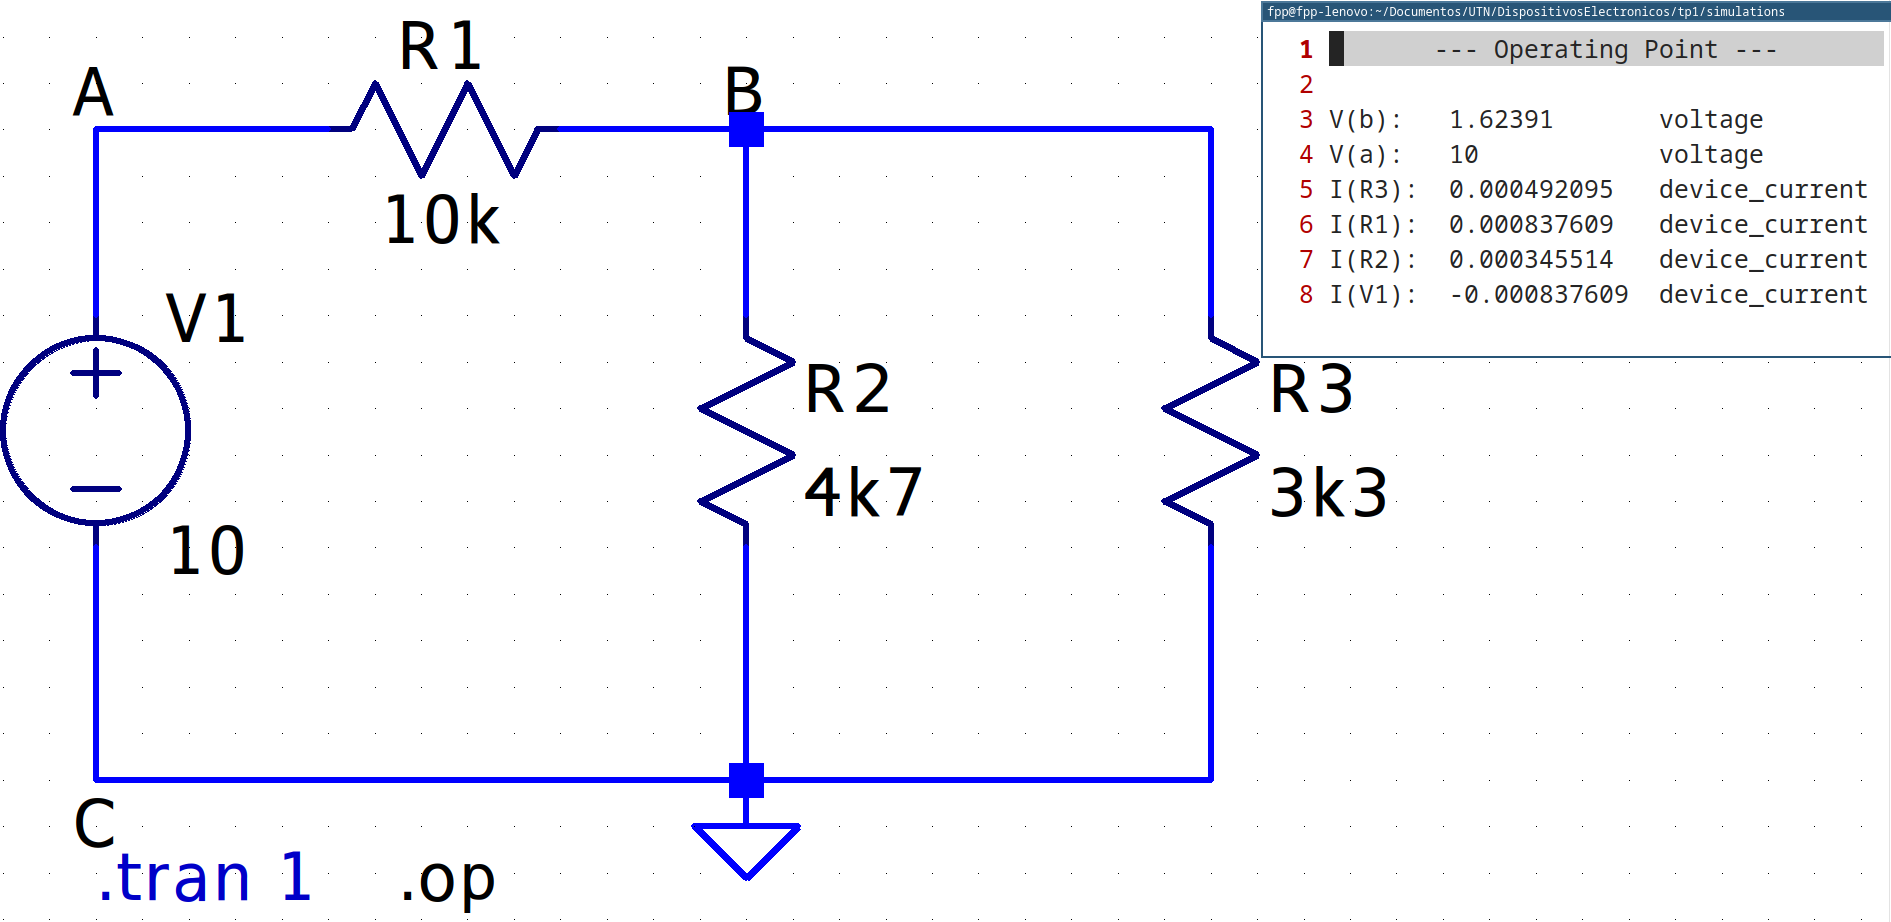
\includegraphics[width=0.8\linewidth]{images/sim_dc.png}

        \caption{Simulacion de punto de operacion del circuito.}
      \end{figure}

      \section{Implementacion y Mediciones}


\end{document}
